% generated by benchmark/make_tables_E.jl from results/E_suite_*.tsv
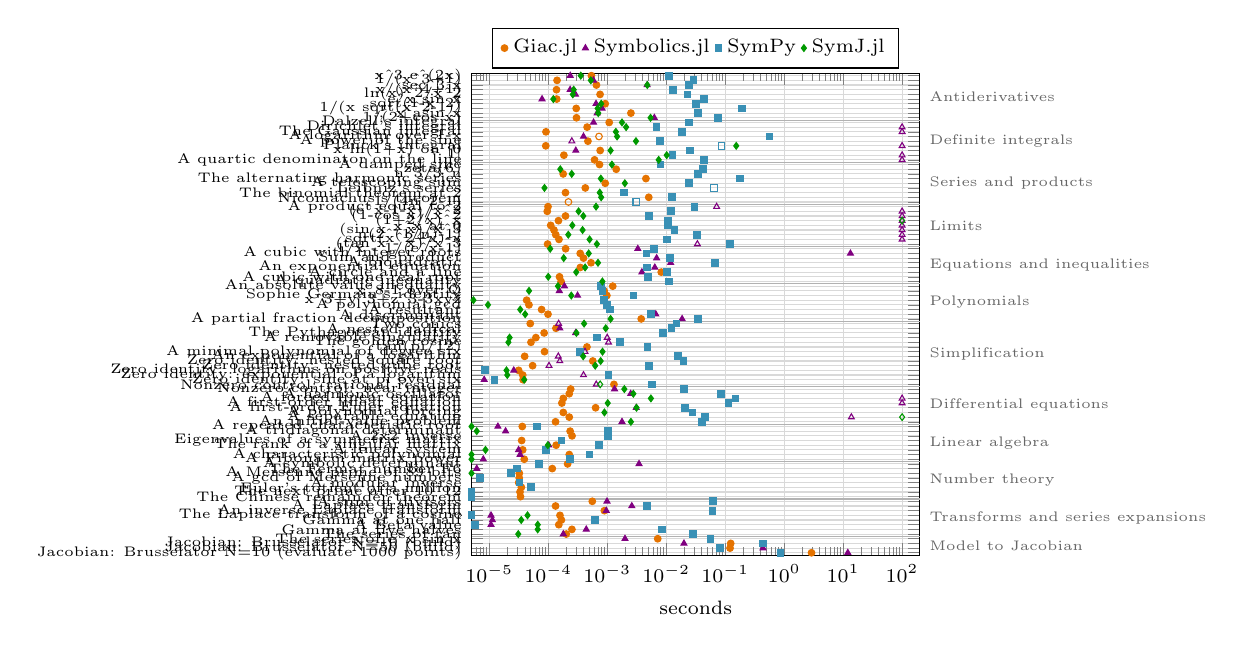
\begin{tikzpicture}
\begin{axis}[xmode=log, width=0.60\textwidth, height=7.7cm,
  xmin=5e-6, xmax=200, xlabel={seconds}, ytick={1,...,103}, y dir=reverse, ymin=0.5, ymax=103.5,
  yticklabels={x\^{}3 e\^{}(2x),1/(x\^{}3+1),sec\^{}3 x,x/(x\^{}4+1),ln(x)\^{}2/x\^{}2,e\^{}x sin x,sqrt(1-x\^{}2),1/(x sqrt(x\^{}2-1)),x asin x,1/(2+cos x),Dalzell's integral,Dirichlet's integral,The Gaussian integral,A logarithm over 1-x,A power of the sine,Planck's integral,x ln(1+x) on [0,1],A quartic denominator on the line,A damped sine,zeta(6),n\^{}3/3\^{}n,The alternating harmonic series,A telescoping sum,Leibniz's series,The binomial theorem at 2,Nicomachus's theorem,1/(4n\^{}2-1),A product equal to 2,(e\^{}x-1-x)/x\^{}2,(1-cos x)/x\^{}2,(1+2/x)\^{}x,x\^{}x at 0,(sin x - x)/x\^{}3,n(2\^{}(1/n)-1),sqrt(x\^{}2+x)-x,(tan x - x)/x\^{}3,1/x - 1/(e\^{}x-1),A cubic with integer roots,Sum and product,A biquadratic,An exponential equation,A circle and a line,A cubic with one real root,A quadratic inequality,An absolute value inequality,x\^{}8-1 over Q,Sophie Germain's identity,x\^{}3+y\^{}3+z\^{}3-3xyz,A polynomial gcd,A resultant,A discriminant,A partial fraction decomposition,Two conics,A nested radical,The Pythagorean identity,A removable singularity,The golden cosine,tan(pi/12),A minimal polynomial of degree six,An exponential of a logarithm,Zero identity: nested square root,Zero identity: nested cube root,Zero identity: logarithms on positive reals,Zero identity: exponential of a logarithm,Zero identity: sine at pi over six,Nonzero control: rational residual,Nonzero control: near integer,A harmonic oscillator,A forced linear equation,A first-order linear equation,A first-order Euler equation,A polynomial forcing,A separable equation,An initial-value problem,A repeated characteristic root,A tridiagonal determinant,A 2x2 inverse,Eigenvalues of a symmetric matrix,The rank of a singular matrix,A linear system,A characteristic polynomial,A Fibonacci matrix power,A symbolic determinant,The Fermat number F6,A Mersenne prime of 89 bits,A gcd of Mersenne numbers,A modular inverse,Euler's totient of a million,The next prime after 10\^{}12,The Chinese remainder theorem,A sum of divisors,A Laplace transform,An inverse Laplace transform,The Laplace transform of a cosine,Gamma at one half,A Beta value,Gamma at five halves,The series of tan,The series of e\^{}x sin x,Jacobian: Brusselator N=10 (build),Jacobian: Brusselator N=50 (build),Jacobian: Brusselator N=10 (evaluate 1000 points),Jacobian: Brusselator N=50 (evaluate 1000 points)}, yticklabel style={font=\tiny}, tick label style={font=\scriptsize},
  xlabel style={font=\scriptsize}, grid=major, grid style={gray!30}, legend style={font=\scriptsize, at={(0.5,1.01)}, anchor=south, legend columns=4},
  clip=false, every axis plot/.append style={only marks}]
\addplot[mark=*, mark size=1.2pt, color=orange!90!black] coordinates {(0.000539,1)(0.000141,2)(0.000656,3)(0.000138,4)(0.000756,5)(0.000139,6)(0.000925,7)(0.000298,8)(0.00252,9)(0.000301,10)(0.00108,11)(0.000456,12)(9.15e-05,13)(0.00047,15)(9.08e-05,16)(0.000759,17)(0.000184,18)(0.00061,19)(0.00074,20)(0.00142,21)(0.000179,22)(0.00453,23)(0.000924,24)(0.000425,25)(0.000196,26)(0.00506,27)(9.91e-05,29)(9.62e-05,30)(0.000196,31)(0.000149,32)(0.00011,33)(0.000125,34)(0.000134,35)(0.000152,36)(9.76e-05,37)(0.000197,38)(0.000348,39)(0.000396,40)(0.000531,41)(0.00035,42)(0.00824,43)(0.000155,44)(0.000165,45)(0.00124,46)(0.000887,47)(0.000986,48)(4.3e-05,49)(4.71e-05,50)(7.71e-05,51)(9.9e-05,52)(0.00377,53)(4.95e-05,54)(0.000135,55)(8.51e-05,56)(6.17e-05,57)(5.09e-05,58)(0.000453,59)(8.64e-05,60)(3.98e-05,61)(0.000569,62)(5.43e-05,63)(3.15e-05,64)(3.69e-05,65)(3.74e-05,66)(0.0013,67)(0.00024,68)(0.000227,69)(0.00018,70)(0.00017,71)(0.000635,72)(0.00018,73)(0.000227,74)(0.000133,75)(3.63e-05,76)(0.000235,77)(0.000253,78)(3.54e-05,79)(0.000136,80)(3.69e-05,81)(0.000227,82)(3.92e-05,83)(0.000213,84)(0.000117,85)(3.23e-05,86)(3.22e-05,87)(3.15e-05,88)(3.5e-05,89)(3.32e-05,90)(3.38e-05,91)(0.000558,92)(0.000133,93)(0.000894,94)(0.000158,95)(0.000167,96)(0.000151,97)(0.000252,98)(0.000202,99)(0.00718,100)(0.124,101)(0.121,102)(2.91,103)};
\addlegendentry{Giac.jl}
\addplot[mark=o, mark size=1.2pt, color=orange!90!black, forget plot] coordinates {(0.000725,14)(0.00022,28)};
\addplot[mark=triangle*, mark size=1.2pt, color=violet] coordinates {(0.000236,1)(0.000583,2)(0.00475,3)(0.000235,4)(0.000289,5)(7.85e-05,6)(0.000646,7)(0.000818,8)(0.000675,9)(0.00629,10)(0.000586,11)(0.000396,14)(0.000293,17)(0.0033,38)(13.3,39)(0.00688,40)(0.0119,41)(0.00641,42)(0.00387,43)(0.000188,46)(0.000154,47)(0.000314,48)(0.00666,52)(0.0186,53)(0.000157,55)(0.000291,56)(2.6e-05,64)(8.2e-06,66)(0.00133,68)(0.0025,69)(0.0031,72)(0.00178,75)(1.4e-05,76)(1.89e-05,77)(0.000102,80)(3.14e-05,81)(3.33e-05,82)(7.93e-06,83)(0.00346,84)(6.13e-06,85)(0.000991,92)(0.00261,93)(0.000964,94)(1.07e-05,95)(1.13e-05,96)(1.07e-05,97)(0.000441,98)(0.00018,99)(0.002,100)(0.02,101)(0.438,102)(12,103)};
\addlegendentry{Symbolics.jl}
\addplot[mark=triangle, mark size=1.2pt, color=violet, forget plot] coordinates {(100,12)(100,13)(0.000251,15)(100,16)(100,18)(100,19)(0.0716,29)(100,30)(100,31)(100,32)(100,33)(100,34)(100,35)(100,36)(0.0338,37)(0.00015,54)(0.000999,57)(0.00105,58)(0.00042,60)(0.000148,61)(0.000157,62)(0.000103,63)(0.000396,65)(0.000651,67)(100,70)(100,71)(13.8,74)};
\addplot[mark=square*, mark size=1.2pt, color=cyan!70!black] coordinates {(0.011,1)(0.0289,2)(0.0245,3)(0.0131,4)(0.0229,5)(0.0434,6)(0.0319,7)(0.195,8)(0.0341,9)(0.0762,10)(0.0242,11)(0.00683,12)(0.0185,13)(0.566,14)(0.00785,15)(0.0252,17)(0.0128,18)(0.0432,19)(0.00799,20)(0.0426,21)(0.0348,22)(0.179,23)(0.0241,24)(0.0019,26)(0.0127,27)(0.0303,29)(0.0119,30)(0.00518,31)(0.0106,32)(0.0106,33)(0.0138,34)(0.0333,35)(0.0103,36)(0.12,37)(0.00613,38)(0.00464,39)(0.0117,40)(0.0663,41)(0.00476,42)(0.0103,43)(0.00488,44)(0.011,45)(0.000781,46)(0.000833,47)(0.00279,48)(0.000883,49)(0.000999,50)(0.00111,51)(0.00545,52)(0.035,53)(0.0149,54)(0.0123,55)(0.00892,56)(0.000674,57)(0.00165,58)(0.00481,59)(0.000346,60)(0.0159,61)(0.0196,62)(0.00511,63)(8.5e-06,64)(0.00105,65)(1.22e-05,66)(0.0058,67)(0.0201,68)(0.084,69)(0.15,70)(0.114,71)(0.0206,72)(0.0278,73)(0.0455,74)(0.0406,75)(6.38e-05,76)(0.00103,77)(0.00103,78)(0.000168,79)(0.000716,80)(9.27e-05,81)(0.000502,82)(0.000232,83)(7.02e-05,84)(2.99e-05,85)(2.36e-05,86)(6.97e-06,87)(3.25e-05,88)(5.16e-05,89)(5e-06,90)(5e-06,91)(0.0621,92)(0.00475,93)(0.0607,94)(5e-06,95)(0.00062,96)(5.7e-06,97)(0.00856,98)(0.0285,99)(0.0566,100)(0.441,101)(0.0811,102)(0.863,103)};
\addlegendentry{SymPy}
\addplot[mark=square, mark size=1.2pt, color=cyan!70!black, forget plot] coordinates {(0.0866,16)(0.0647,25)(0.00311,28)};
\addplot[mark=diamond*, mark size=1.2pt, color=green!60!black] coordinates {(0.000356,1)(0.000527,2)(0.00478,3)(0.00027,4)(0.000261,5)(0.000122,6)(0.000791,7)(0.000688,8)(0.000705,9)(0.00543,10)(0.00178,11)(0.00209,12)(0.0014,13)(0.00147,14)(0.00307,15)(0.154,16)(0.00114,17)(0.0102,18)(0.00745,19)(0.0012,20)(0.00016,21)(0.00025,22)(0.000779,23)(0.00199,24)(8.63e-05,25)(0.000746,26)(0.00079,27)(0.000646,29)(0.000327,30)(0.000393,31)(0.000256,33)(0.000382,34)(0.000219,35)(0.000502,36)(0.000667,37)(0.000108,38)(0.000485,39)(0.000183,40)(0.000697,41)(0.000422,42)(0.000298,43)(0.0001,44)(0.000828,45)(0.000146,46)(4.72e-05,47)(0.000246,48)(5.39e-06,49)(9.5e-06,50)(3.35e-05,51)(4.06e-05,52)(0.00114,53)(0.000405,54)(0.000943,55)(0.0003,56)(2.21e-05,57)(2.11e-05,58)(0.000832,60)(0.000391,61)(0.000774,62)(0.000626,63)(1.96e-05,64)(2.02e-05,65)(3.91e-05,66)(0.00195,68)(0.00277,69)(0.0055,70)(0.00102,71)(0.00314,72)(0.000896,73)(0.00252,75)(5e-06,76)(6.13e-06,77)(9.83e-05,80)(8.63e-06,81)(5e-06,82)(5e-06,83)(5e-06,86)(4.45e-05,95)(3.48e-05,96)(6.63e-05,97)(6.62e-05,98)(3.1e-05,99)};
\addlegendentry{SymJ.jl}
\addplot[mark=diamond, mark size=1.2pt, color=green!60!black, forget plot] coordinates {(100,32)(0.00076,67)(100,74)};
\node[anchor=west, font=\tiny, text=gray!80!black] at (axis cs:200,5.5) {Antiderivatives};
\draw[gray!60] (axis cs:5e-6,10.5) -- (axis cs:200,10.5);
\node[anchor=west, font=\tiny, text=gray!80!black] at (axis cs:200,15.0) {Definite integrals};
\draw[gray!60] (axis cs:5e-6,19.5) -- (axis cs:200,19.5);
\node[anchor=west, font=\tiny, text=gray!80!black] at (axis cs:200,24.0) {Series and products};
\draw[gray!60] (axis cs:5e-6,28.5) -- (axis cs:200,28.5);
\node[anchor=west, font=\tiny, text=gray!80!black] at (axis cs:200,33.0) {Limits};
\draw[gray!60] (axis cs:5e-6,37.5) -- (axis cs:200,37.5);
\node[anchor=west, font=\tiny, text=gray!80!black] at (axis cs:200,41.5) {Equations and inequalities};
\draw[gray!60] (axis cs:5e-6,45.5) -- (axis cs:200,45.5);
\node[anchor=west, font=\tiny, text=gray!80!black] at (axis cs:200,49.5) {Polynomials};
\draw[gray!60] (axis cs:5e-6,53.5) -- (axis cs:200,53.5);
\node[anchor=west, font=\tiny, text=gray!80!black] at (axis cs:200,60.5) {Simplification};
\draw[gray!60] (axis cs:5e-6,67.5) -- (axis cs:200,67.5);
\node[anchor=west, font=\tiny, text=gray!80!black] at (axis cs:200,71.5) {Differential equations};
\draw[gray!60] (axis cs:5e-6,75.5) -- (axis cs:200,75.5);
\node[anchor=west, font=\tiny, text=gray!80!black] at (axis cs:200,79.5) {Linear algebra};
\draw[gray!60] (axis cs:5e-6,83.5) -- (axis cs:200,83.5);
\node[anchor=west, font=\tiny, text=gray!80!black] at (axis cs:200,87.5) {Number theory};
\draw[gray!60] (axis cs:5e-6,91.5) -- (axis cs:200,91.5);
\node[anchor=west, font=\tiny, text=gray!80!black] at (axis cs:200,95.5) {Transforms and series expansions};
\draw[gray!60] (axis cs:5e-6,99.5) -- (axis cs:200,99.5);
\node[anchor=west, font=\tiny, text=gray!80!black] at (axis cs:200,101.5) {Model to Jacobian};
\end{axis}
\end{tikzpicture}
